\section{Underground logbook: Stagger Lee, Big Rock's Big Brother}

\margininbox{Big Rock Candy Mountain}{
     \begin{itemize}
    \item Dan Greenwald
    \item Dave Wilson
    \end{itemize}}{\explo}

\textbf{3/8/12 18:00 Dan}

Dave + Dan off to \passage{Big Rock Candy Mountain}. Back approx 20-00.

\textbf{3/8/12 23:55}

A predictably faff-heavy start meant we didn't get underground till
about 3:30. Down at \passage{X-Ray} at 6, stopping to faff + fettle + wake the lighter sleepers of the night train (sorry).

Got to \passage{Big Rock} and I started down with the drill etc to find glory. In fact, I found a scary-arse traverse which I got about halfway across. Dave came down to join me and we made a tactical decision to approach the remainder tomorrow, also ensuring we got back before buffalo-hour. Meaty, cheesy, soupy smash consumed with relish.

Night train got out of the tent with surprising eagerness.

Comf donned, Jarv + Ollie returned from the deep. Great to be back at camp (finally). Sleep now. Where is the whiskey?

\name{Dan Greenwald}

\textbf{5/8/12 10:30}

Great day yesterday -- finished the traverse to \passage{Big Rock}'s big brother. Very wet, quite sketchy but really fun. There's a new way up from the bottom of \passage{Big Rock}, so no one needs to go there again. Except to derig it. The pitch on the other side is huge. We didn't get very far down, there's $\approx$ 60 m of 9 ½ mm at the top for someone else to enjoy. To the surface!

\name{Dan Greenwald}

\textbf{7/8/12 8:30 am}

\margininbox{Stagger Lee}{
     \begin{itemize}
    \item Tim Osborne
    \item Tharatorn Supasiti
    \end{itemize}}{\explo}

Tim and I (dream team) went for the glory at \passage{Big Rock} (soon to be
called \passage{Stagger Lee}). After arriving at the camp around 830pm, faffed around cooking, eating, drinking. We soon found that the camp was without a drill bit. Nevermind, old style bolting mission.

Set off around 10pm to \passage{Big Rock}. After the first bolt we soon have a fucked driver. However we managed to bolt down to the second level, where Tim braved the drizzle (like \passage{Zimmer}) and tried to bolt down to the lower level.


\begin{marginfigure}
\checkoddpage \ifoddpage \forcerectofloat \else \forceversofloat \fi
\centering
 \frame{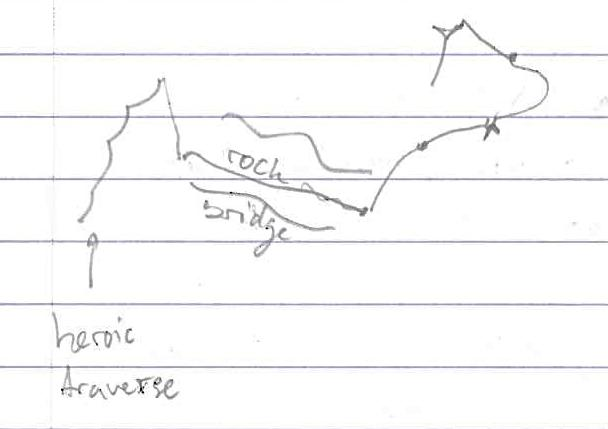
\includegraphics[width=\linewidth]{2012/staggerlee/bigrocktraverse.jpg}} 
 \caption{A sketch of traversing in \passage{Big Rock Candy Mountain}. \pen{Tharatorn Supasiti}}
 \label{bcrm traverse}
\end{marginfigure}


Going back tomorrow to go down and survey!

Hopefully, string of bad luck won't continue\ldots{}

\name{Thara Supasiti}



\fullwidthbox{The Raptured}{

\textit{8/8/12 16:45}

Well, Jonath and myself set off from the Bivi yesterday and I realised at the entrance that I just wasn't that keen, we set off anyway thinking that I was being silly and the enthusiasm would soon set in. Unfortunately in the \passage{Urinal Series} the fun had not begun, dear dear Jonath was lovely and made me feel ok so we got to the big pitches and things got better. It wasn't any sort of extreme fear, just an unwillingness to be in the fun caving state. We eventually got to camp and set off to \passage{Xanadu}/\passage{Euphrates} to connect the survey which was v. grim. Jonny tried to bolt the pitch which is v. blowing \& cold but the rock is shit and kept breaking. We headed back to camp but I still wasn't comfortable and was very shaky. After lots of dancing, which me \& Jonath happened to be very skilled at, we went to bed.

Today I wasn't keen to go as far as \passage{Atlantis} but really wanted to for Jonny so just as we were about to set off Jonny realises that he's also raptured and just wanted to head out. Much to Gergely's confusion we realised that neither of us were super enthused then we should cut our losses and head out, freeing up bed space for the mega-keen. We still accomplished the \passage{Xanadu}/\passage{Euphrates} connection and have had a pleasant time. We shall
definitely be coming back super-pumped and ready for action, just this time wasn't meant to be.

Peace out

\name{Kate x} 

Besides I quite need a shit and I have sworn to never poo underground.}


\textbf{8/8/12 4pm Thara}

Officially, we (Tim and I) are the connection makers (loopers).

We surveyed from the bottom of \passage{Big Rock} because we couldn't find any PSS station. Hopefully, we make a connection at the right place there.

Continued bolting down the pitch Dan planned to descend. Tim put two quick bolts (thanks to drill bit) and dropped down to the bottom which is filled with human-size boulders stacked Jenga-like.

We looked for the obvious chamber by following the streamway.

3 bolts and we were at the botto. Followed the stream for a few more minutes until we realised that we were in \passage{Soda Streamway} -- CONNECTION! Again.

Slowly surveyed the rest and derigged all the ropes.

Three possible leads (not that exciting):

\begin{enumerate}
\def\labelenumi{\arabic{enumi}.}
\item
  Window at the same level as rock wall
\item
  Window at the same level as traverse ledge
\item
  Window \textasciitilde 3 metres above the bottom
\end{enumerate}


\begin{marginfigure}
\checkoddpage \ifoddpage \forcerectofloat \else \forceversofloat \fi
\centering
 \frame{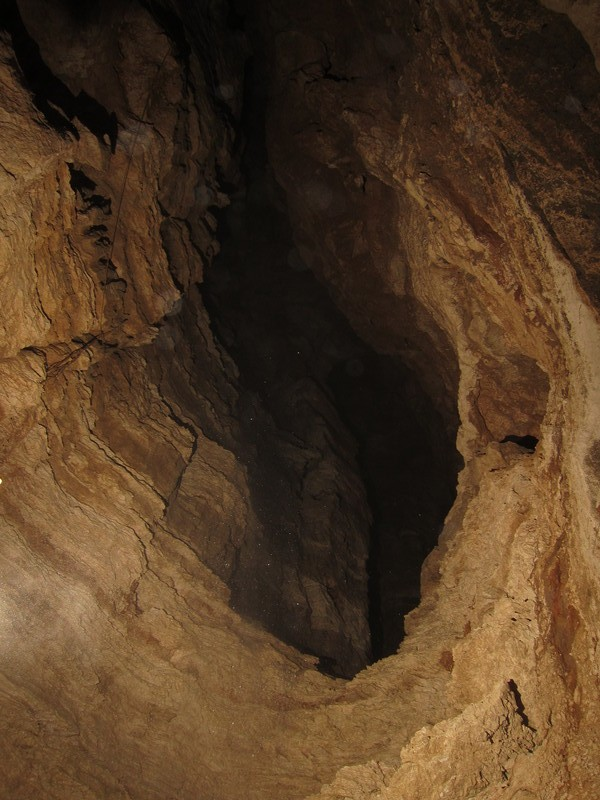
\includegraphics[width=\linewidth]{2012/staggerlee/2014-07-31_0626_JarvistMooreFrost_S95_IMG_4682_BigRock-LookingUpPitchFromBottom--orig.jpg}} 
 \caption{Looking up \passage{Big Rock Candy Mountain} in 2014 (the rope disappears into the abyss to the left). \pic{Jarvist Frost}}
 \label{big rock candy mountain}
\end{marginfigure}


The first two seem to head back into the rifts already explored. The third seems to head towards \passage{Balamory}.

\name{Thara Supasiti}
